%% lfgw: 2.19 Lyrik-Satz


%% !TEX root = lfgw.tex

\RequirePackage{iftex}
\RequireLuaTeX
\RequirePackage{luatex85}

\documentclass[%
   ibycus,polutonikogreek,english,french,latin,ngerman,%global definiert!
   %%%draft=false,%
   fontsize=11pt,%
   paper=17cm:24cm,%
   DIV=13,%
   listof=totoc,%
   bibliography=totoc,%
   pagesize%
   ]{scrbook}

\KOMAoption{bibliography}{leveldown}

\usepackage{yfonts}
\usepackage{textgreek}
\usepackage{cjhebrew}[2017/03/06]
\usepackage{amsmath,amssymb} % für forrest
%%%\usepackage{textcomp}
\usepackage{unicode-math}
\usepackage{fontspec}
\defaultfontfeatures{Ligatures=TeX,Scale=MatchLowercase}
%\newfontfamily\GFSDidot{GFS Didot}
\newcommand\gkk[1]{%{\GFSDidot
#1}

\usepackage[]{babel}
%\usepackage[ngerman,noftligs]{selnolig}
%%%\setmainfont{Libertinus Serif} %reicht auch, unten evtl. besser wegen SB
\setmainfont{libertinusserif}[
   Extension = {.otf},
   UprightFont = {*-regular}, ItalicFont = {*-italic},
   BoldFont = {*-bold}, BoldItalicFont = {*-bolditalic},%
   FontFace = {sb}{\updefault}{*-semibold},%
   FontFace = {sb}{it}{*-semibolditalic}]%
\setsansfont{Libertinus Sans}
\setmonofont[Scale=MatchLowercase,FakeStretch=0.85]{DejaVu Sans}%das wird für Griechisch in Codebeispielen gebraucht
\setmathfont{Libertinus Math}
\makeatletter
\newcommand*\sustyle{\addfontfeatures{VerticalPosition=Superior}}
\DeclareTextFontCommand{\textsu}{\sustyle}
\def\@makefnmark{\hbox{\sustyle\@thefnmark}}
\makeatother
\DeclareTextCommandDefault{\textborn}{{\char"002A}}
\DeclareTextCommandDefault{\textdied}{{\char"2020}}
\usepackage[% microtype
   final,%
   tracking=smallcaps,%
   expansion=alltext,%
   protrusion=true%
   ]{microtype}%
\SetTracking{encoding=*,shape=sc}{50}%
\UseMicrotypeSet[protrusion]{basicmath} % disable protrusion for tt fonts

\usepackage[headsepline]{scrlayer-scrpage}
\clearscrheadfoot
\ihead{\headmark}
\ohead{\pagemark}
\pagestyle{scrheadings}

\usepackage[autostyle]{csquotes}
\usepackage[newcommands]{ragged2e}

\usepackage{graphicx}
\graphicspath{{bilder/}}

\usepackage{grffile}
\usepackage[a4,center,cross]{crop}

\usepackage{listings}
\lstdefinestyle{listinglfgw}{%
  inputencoding=utf8,
  extendedchars=true,
  language=[LaTeX]{TeX},
  numbers=left, 
  %stepnumber=3,
  numbersep=5pt, 
  numberfirstline=false,  
  numberstyle=\tiny\textsf,
  basicstyle=\ttfamily\footnotesize,
  keywordstyle=\bfseries,%
  texcsstyle=*\ttfamily\footnotesize\bfseries,%
  %frame=tlrb,
  breaklines=true,
  breakatwhitespace=true,
  breakindent=5pt,
  %postbreak=\mbox{$\hookrightarrow$},
  escapeinside={*@}{@*},
  %showstringspace=false, 
  captionpos=b,
  upquote=true,
  %%%classoffset=0,
  morekeywords={%
  %a
  addbibresource,addplot,Afootnote,alteSeite,autocite,autopar,answerline,alertblock,
  %b
  beginnumbering,Bfootnote,biblerefformat,biblerefmap,biblerefstyle,bonuspointpoints,bibleref,block,
  %c
  Cfootnote,chapter,chbpword,chpword,chpgword,chqword,chsword,chtword,citeauthor,cites,citetitle,columnrulewidth,Columns,columnsposition, center,
  chronology,columns,
  %d
  draw,dictum,deffootnote,deffootnote,description,
  %e
  edtext,endnumbering,enquote,enumi,example,exampleblock,
  %f
  firstlinenum,firstlinenumR,firstpageheadrule,footcite,footcites,footfullcite,fullcite,fillwithgrid,fillwithlines,fillwithdottedlines,Forest,Forest*,
  footnotemargin,fillwithlines, fillwithgrid,
  %h
  hpword,hqword,hsword,htword,hypertarget,hyperlink,hideallsubsection,
  %i
  includegraphics,includeonlyframes,ibibleref,invisible,
  %l
  Lcolwidth,ledsidenote,lemma,linenumincrement,linenumincrementR,
  %m
  msdata,mode,maketitle,multifootsep,
  %n
  newfontface,newfontfamily,node,
  %o
  only,onslide,
  %p
  Pages,parencite,parencites,part,pend,pibibleverse,pbibleverse,pointpoints,printbibheading,printbibliography,printindex,pstart,pgfimage,pgfusepath,
  pgfplothandlerlineto,pgfplotsset,pgfplotxyfile,pbibleref,pibibleref,pgf-pie,plain,
  %q
  quell,question,quote,quotaion,
  %r
  Rcolwidth,reledmac,
  %s
 selectlanguage,setlength,setmainfont,setmonofont,setmsdatalabel,setromanfont,setsansfont,smartcite,smartcites,solutiontitle,setbeamerfont,setbeamercovered,subsection,subsection*,subsubsection,subtitle,solution,solutionorgrid,
  %t
  text,textborn,textcite,textcites,textdelta,textDelta,textdied,texteuro,textgamma,textGamma,textmarried,textsubscript,thealteSeite,tableofcontents,th,TH,
  textalpha, textbeta, textgamma, textdelta, textepsilon, textzeta, texteta, texttheta, textiota, textkappa, textlambda, textmu, textnu,
  textxi, textomikron, textpi, textrho, textsigma, texttau, textupsilon, textphi, textchi,  textpsi, textomega,
  textAlpha, textBeta, textGamma, textDelta, textEpsilon, textZeta, textEta, textTheta, textIota, textKappa, textLambda, textMu, textNu,
  textXi, textOmikron, textPi, textRho, textSigma, textTau, textUpsilon, textPhi, textChi,  textPsi, textOmega, twocolumn,
  %u
  usetheme,usecolortheme,usebackgroundtemplate,useforestlibrary,usepackage,usetikzlibrary,
  %v
  vari,verse,
  %x
  Xafternumber,Xarrangement,Xlemmaseparator,Xinplaceoflemmaseparator,Xinplaceofnumber,Xnonbreakableafternumber,Xnotenumfont,Xnumberonlyfirstinline,Xnumberonlyfirstintwolines,Xsymlinenum,Xtwolines,Xtwolinesbutnotmore,Xtxtbeforenotes
  },   
  literate=
  {á}{{\'a}}1 {é}{{\'e}}1 {í}{{\'i}}1 {ó}{{\'o}}1 {ú}{{\'u}}1
  {Á}{{\'A}}1 {É}{{\'E}}1 {Í}{{\'I}}1 {Ó}{{\'O}}1 {Ú}{{\'U}}1
  {à}{{\`a}}1 {è}{{\`e}}1 {ì}{{\`i}}1 {ò}{{\`o}}1 {ù}{{\`u}}1
  {À}{{\`A}}1 {È}{{\'E}}1 {Ì}{{\`I}}1 {Ò}{{\`O}}1 {Ù}{{\`U}}1
  {ä}{{\"a}}1 {ë}{{\"e}}1 {ï}{{\"i}}1 {ö}{{\"o}}1 {ü}{{\"u}}1
  {Ä}{{\"A}}1 {Ë}{{\"E}}1 {Ï}{{\"I}}1 {Ö}{{\"O}}1 {Ü}{{\"U}}1
  {â}{{\^a}}1 {ê}{{\^e}}1 {î}{{\^i}}1 {ô}{{\^o}}1 {û}{{\^u}}1
  {Â}{{\^A}}1 {Ê}{{\^E}}1 {Î}{{\^I}}1 {Ô}{{\^O}}1 {Û}{{\^U}}1
  {œ}{{\oe}}1 {Œ}{{\OE}}1 {æ}{{\ae}}1 {Æ}{{\AE}}1 {ß}{{\ss}}1
  {ç}{{\c c}}1 {Ç}{{\c C}}1 {ø}{{\o}}1 {å}{{\r a}}1 {Å}{{\r A}}1
  {€}{{\EUR}}1 {£}{{\pounds}}1
}
\lstset{style=listinglfgw}
  
\usepackage[% tcolorbox
  skins,%
  listings,%
  breakable,%
]{tcolorbox}
\tcbset{%
lfgwstyle/.style={%
    before skip=\baselineskip,
    boxrule=0pt,
    %bottomrule=2pt,
    %toprule=2pt,
    %colframe=black,
    colback=black!5,
    coltitle=white,
    bicolor,
    sharp corners,
    colbacklower=white,
    fonttitle=\sffamily\bfseries,
    breakable,
    %label=#1,
}}


\newtcblisting[auto counter,number within=chapter]{lfgwexample}[1]{%
    lfgwstyle,
    fontupper=\small\ttfamily,
    sidebyside,
    listing and text,
    title={Beispiel \thetcbcounter},
    listing options={style=listinglfgw},
    #1,
%text and listing,
}

\newtcblisting[use counter from=lfgwexample,number within=chapter]{lfgwcode}[1]{%
    lfgwstyle,
    fontupper=\small\ttfamily,
    listing only,
    title={Beispiel \thetcbcounter},
    listing options={style=listinglfgw},
    #1,
}

\newtcblisting[use counter from=lfgwexample,number within=chapter]{lfgwprint}[1]{%
    fontupper=\small,
    lfgwstyle,
    text only,
    title={Beispiel \thetcbcounter},
    listing options={style=listinglfgw},
    #1,
}


\usepackage{showexpl}
%\lstset{explpreset={escapeinside={*@}{@*}}}

\usepackage[pagewise]{lineno}
\usepackage{sidenotes}
\usepackage{multicol}
% Für den Abschnitt über Konstituentenanylyse von C. Römer:
\usepackage[linguistics]{forest}
\forestapplylibrarydefaults{linguistics,edges}
\useforestlibrary{edges}
\makeatletter
\let\pgfmathModX=\pgfmathMod@
\usepackage{pgfplots}%
\pgfplotsset{compat=1.14}
\let\pgfmathMod@=\pgfmathModX
\makeatother
%http://tex.stackexchange.com/questions/328972/presence-of-pgfplots-package-breaks-forest-environment-%w-folder-option-en/329015

% Pakete im Bereich Kapitel 3 - Diagramme zeichnen
\usepackage{tikz}
\usepackage[all]{genealogytree}
\usepackage{chronology}
\usepackage{pgf-pie}
\usetikzlibrary{pgfplots.dateplot}
\usetikzlibrary{mindmap}

\deffootnote[1.5em]{1.5em}{1.5em}{\makebox[1.5em][l]{{\fontseries{sb}\selectfont\thefootnotemark\ }}}

\usepackage{enumitem}			% for simple list modifications
\setlist{leftmargin=*,before=\setlength{\rightmargin}{\leftmargin}}

%\usepackage{parallel}


%- Für Lyrik-Satz, Christine Römer:
\usepackage{verse}
\newcommand\He{\textbackslash\xspace}
\newcommand\Se{$\cup$\xspace} 
\newcommand*{\Zr}{\unskip\textunderscore}
\newcommand\daktylus{\textbackslash$\cup\cup$\xspace} 
\newcommand\anapaest{$\cup\cup$\textbackslash\xspace}

% ------------
\usepackage{runic}
\usepackage{hieroglf}
\usepackage[normalem]{ulem} %%% MS: Wofür? Unterstreichungen sollten vermieden werden! LCB: kann \xout
%\usepackage{letterspace} %%% MS: Wofür. Besser direkt \textls aus dem Microtypepaket
%% ------------------------------------------------------------------------
%%   This is a stand-alone version that only provides the letterspacing
%%   commands. Do not use this package together with the `microtype' package.
%%   Please refer to section 7 of the `microtype' documentation.
%% ------------------------------------------------------------------------ 
\usepackage[hyphens]{url}
\usepackage{hologo}
\usepackage{philex}
\def\fg{}
\usepackage{siunitx} %Supreme typesetting of units
%\sisetup{%
%    tight-spacing=true, %
%    %math-rm=\mathsf, 
%    %		text-rm=\sffamily,
%    detect-all, %Zahlen werden in der aktuellen Schrift angezeigt
%    detect-family,
%    exponent-to-prefix  	= true,%
%    round-mode          	= places,% 
%    round-precision     	= 2,%
%    group-minimum-digits 	= 4, % Für "Tausenderpunkt" --> 1.234 anstatt 1234
%    group-separator			={.},% für "12.345" statt "12 345"
%    %  scientific-notation = engineering, % Use multiples of 3 as exponent
%    locale					=DE, % Typeset numbers and units the German way
%    range-phrase 			={$\times$},%
%    %		zero-decimal-to-integer,%aus "2.0" wird "2"
%    range-units				=single,  % --> 2 x 2 m, - auskommentieren für 2 m x 2 m
%    %%%---------
%%    unit-color=myred,
%}

\usepackage[german]{keystroke}% Computer-Tastatur-Tasten in Anweisungs-Texte zu setzen (z.B. \Shift, \Ctrl, \Spacebar).

\usepackage{imakeidx}
\indexsetup{level = \subsection*, toclevel = subsection, noclearpage, headers = {\indexname}{\indexname}}
\makeindex[                title = {Allgemeiner Index}]
\makeindex[name = pakete,  title = {Verzeichnis der Paketnamen}]
\usepackage[% biblatex
   style=authoryear,  
%  style=historische-zeitschrift, % das am liebsten - aber der geht (bei mir?) nicht!
%  pageref=true,
	backend=biber
	]{biblatex}
\addbibresource{lfgw-bibliographie.bib}
%%%\defbibheading{bibliography}{\addchap{#1}} %%%Besser bei \addchap bleiben

\usepackage{fancyvrb}
\makeatletter
\usepackage[% reledmac
   series={A,B,C},%nur die Apparate A B C aktivieren
   noend,%keine Endotenapparate
   noeledsec%keine eledsections et al.
   %noledgroup%keine ledgroups -- das muss hier auskommentiert werden, damit die minipages funktionieren!
]{reledmac}%
\@ifpackagelater{reledmac}{2017/03/20}{%
   % Package is new enough
}{%
\PackageError{reledmac}{Es wird reledmac >= 2.18.1 benötigt.}%
}
\makeatother
\usepackage{reledpar}

\usepackage{varioref}
\usepackage{hyperxmp}
\usepackage{hyperref}
\hypersetup{					% setup the hyperref-package options
	pdftitle={LaTeX für Geisteswissenschaftler},	% 	- title (PDF meta)
	pdfsubject={Handbuch},% 	- subject (PDF meta)
	pdfauthor={varia},	% 	- author (PDF meta)
	pdfauthortitle={},
	pdfcopyright={Copyright (c) \the\year\. All rights reserved.},
	pdfhighlight=/N,
	pdfdisplaydoctitle=true,
	pdfdate={\the\year-\the\month-\the\day}
	pdflang={de},
   pdfencoding=unicode,   % Sorgt für korrekte Umlaute in den pdf-Lesezeichen - thm
	pdfcaptionwriter={varia},
	pdfkeywords={{LaTeX}, {Geisteswissenschaften}},
	pdfproducer={LuaLaTeX},
	pdflicenseurl={http://creativecommons.org/licenses/by-nc-nd/4.0/},
	plainpages=false,			% 	- 
   colorlinks   = true, %Colours links instead of ugly boxes
   urlcolor     =  blue!50!black, %Colour for external hyperlinks
   linkcolor    = blue, %Colour of internal links
   citecolor   = green!50!black, %Colour of citations
   linktoc=page,
  	pdfborder={0 0 0},			% 	-
	breaklinks=true,			% 	- allow line break inside links
 %   bookmarks=true,
	bookmarksnumbered=true,		%
	bookmarksopenlevel=2,
	bookmarksopen=true,		%
   bookmarksdepth=3,
   pdfdisplaydoctitle,
	final=true	% = true, nur bei web-Dokument!! (wichtig!!)
}
\usepackage{bookmark}%advanced bookmarks
\usepackage[% cleveref
  sort,
  nameinlink
  ]{cleveref}%nach hyperref laden

\crefname{tcb@cnt@lfgwexample}{Beispiel}{Beispiele}
\addto\captionsngerman{%
    \crefformat{lfgwexample}{#2Beispiel\,#1#3}%
    \crefformat{lfgwcode}{#2Beispiel\,#1#3}%
    \crefformat{lfgwprint}{#2Beispiel\,#1#3}%
}

\setkomafont{pagehead}{\normalcolor\normalfont\small\upshape}
\setkomafont{pagenumber}{\normalcolor\normalfont\normalsize\bfseries}

\renewcommand*{\glqq}{\textquotedblleft}
\renewcommand*{\grqq}{\quotedblbase}

\providecommand*{\reledmac}{\mbox{\Package{reledmac}}\xspace}

\providecommand*{\LaTeXTeX}{\hologo{(La)TeX}}
\providecommand*{\AmSLaTeX}{\hologo{AmSLaTeX}}
\providecommand*{\AmSTeX}{\hologo{AmSTeX}}
\providecommand*{\biber}{\hologo{biber}}
\providecommand*{\BibTeX}{\hologo{BibTeX}}
\providecommand*{\BibTeXacht}{\hologo{BibTeX8}}
\providecommand*{\ConTeXt}{\hologo{ConTeXt}}
\let\context\ConTeXt
\providecommand*{\emTeX}{\hologo{emTeX}}
\providecommand*{\eTeX}{\hologo{eTeX}}
\providecommand*{\ExTeX}{\hologo{ExTeX}}
\providecommand*{\HanTheThanh}{\hologo{HanTheThanh}}
\providecommand*{\iniTeX}{\hologo{iniTeX}}
\providecommand*{\KOMAScript}{\hologo{KOMAScript}}
\providecommand*{\LaTeX}{\hologo{LaTeX}}
\providecommand*{\LaTeXe}{\hologo{LaTeX2e}}
\providecommand*{\LaTeXIII}{\hologo{LaTeX3}}
\providecommand*{\LaTeXML}{\hologo{LaTeXML}}
\providecommand*{\LuaLaTeX}{\hologo{LuaLaTeX}}
\let\lualatex\LuaLaTeX
\providecommand*{\LuaTeX}{\hologo{LuaTeX}}
\let\luatex\LuaTeX
\providecommand*{\LyX}{\hologo{LyX}}
\providecommand*{\METAFONT}{\hologo{METAFONT}}
\let\MF\METAFONT
\providecommand*{\MetaFun}{\hologo{MetaFun}}
\providecommand*{\METAPOST}{\hologo{METAPOST}}
\providecommand*{\MetaPost}{\hologo{MetaPost}}
\let\MP\METAPOST
\providecommand*{\MiKTeX}{\hologo{MiKTeX}}
\providecommand*{\NTS}{\hologo{NTS}}
\providecommand*{\OzMF}{\hologo{OzMF}}
\providecommand*{\OzMP}{\hologo{OzMP}}
\providecommand*{\OzTeX}{\hologo{OzTeX}}
\providecommand*{\OzTtH}{\hologo{OzTth}}
\providecommand*{\PCTeX}{\hologo{PCTeX}}
\providecommand*{\pdfTeX}{\hologo{pdfTeX}}
\let\pdftex\pdfTeX
\providecommand*{\pdfLaTeX}{\hologo{pdfLaTeX}}
\let\pdflatex\pdfLaTeX
\providecommand*{\PiC}{\hologo{PiC}}
\providecommand*{\PiCTeX}{\hologo{PiCTeX}}
\providecommand*{\plainTeX}{\hologo{plainTeX}}
\providecommand*{\SageTeX}{\hologo{SageTeX}}
\providecommand*{\SLiTeX}{\hologo{SLiTeX}}
\providecommand*{\teTeX}{\hologo{teTeX}}
\providecommand*{\TeXivht}{\hologo{TeX4ht}}
\providecommand*{\TTH}{\hologo{TTH}}
\providecommand*{\virTeX}{\hologo{virTeX}}
\providecommand*{\VTeX}{\hologo{VTeX}}
\providecommand*{\XeLaTeX}{\hologo{XeLaTeX}}
\providecommand*{\XeTeX}{\hologo{XeTeX}}
%%
\newcommand\BibTool{\textsc{Bib\hskip-.1em
      T\hskip-.15emo\hskip-.05emo\hskip-.05eml}\xspace}
\providecommand*{\TikZ}{\textsf{Ti\textit{k}Z}}
%\providecommand*{\pgf/tikz}{\textsf{pgf/Ti\textit{k}Z}}
\def\pgf/tikz{\textsf{pgf/Ti\textit{k}Z}}
\providecommand*{\ALEPH}{\ensuremath{\aleph}}

\providecommand\eV{e.V\kern-0.18em\@ifnextchar.{}{.}\kern0.18em}
\providecommand\dante{\mbox{DANTE~\eV}}
\providecommand\Dante{DANTE,
   Deutschsprachige Anwendervereinigung \TeX~\eV}
\providecommand\DTK{Die \TeX\-ni\-sche Ko\-m{\"o}\-die}
\providecommand\PS{Post\-Script}
\providecommand\TUG{\TeX{} Users Group}
\providecommand\TUGboat{\textsl{TUGboat}}
\let\DANTE\dantelogo
\providecommand*{\TeXLive}{\TeX{}Live}

\def\BibLaTeX{Bib\hologo{LaTeX}}
\let\biblatex\BibLaTeX
\providecommand*{\CTAN}{\texttt{CTAN}\xspace}

\providecommand*{\prog}[1]{\texttt{#1}}
\let\Program\prog

\providerobustcmd*{\paket}[2][]{\textsf{#2}\index[pakete]{\if$#1$#2\else#1\fi}}
\let\Package\paket%zwecks kompatibilität mit DTK
\let\Paket\paket
\newcommand*{\opt}[1]{\texttt{#1}}
\newcommand*{\file}[1]{\texttt{#1}}
\newcommand*{\env}[1]{\texttt{#1}}

\makeatletter
\DeclareRobustCommand\cs[1]{\texttt{\bfseries\char`\\#1}}
\DeclareRobustCommand\meta[1]{%
   \ensuremath\langle
   \ifmmode \expandafter \nfss@text \fi
   {%
      \meta@font@select
      \edef\meta@hyphen@restore
      {\hyphenchar\the\font\the\hyphenchar\font}%
      \hyphenchar\font\m@ne
      \language\l@nohyphenation
      #1\/%
      \meta@hyphen@restore
   }\ensuremath\rangle
}
\def\marg{\@ifstar{\@@marg}{\@marg}}
\providecommand\@marg[1]{%
   {\ttfamily\mdseries\char`\{}\meta{#1}{\ttfamily\mdseries\char`\}}}
\providecommand\@@marg[1]{%
   {\ttfamily\mdseries\char`\{}{\mdseries #1}{\ttfamily\mdseries\char`\}}}
\def\oarg{\@ifstar{\@@oarg}{\@oarg}}
\providecommand\@oarg[1]{%
   {\ttfamily\mdseries[}\meta{#1}{\ttfamily\mdseries]}}
\providecommand\@@oarg[1]{%
   {\ttfamily\mdseries[}{#1}{\ttfamily\mdseries]}}
\providecommand\parg[1]{%
   {\ttfamily\mdseries(}\meta{#1}{\ttfamily\mdseries)}}
\def\meta@font@select{\itshape\mdseries}
\makeatother

\tolerance 1414
\hbadness 1414
\emergencystretch 1.5em
\hfuzz 0.3pt
\widowpenalty=10000
\displaywidowpenalty=10000
\clubpenalty=5000
\interfootnotelinepenalty=9999
\brokenpenalty=2000
\vfuzz \hfuzz
%%%\raggedbottom


% Autorkennung:   Wie soll's aussehen?
\providecommand{\autor}[1]{\hfill\textbf{#1}}

\endinput



%\usepackage{verse}
%\newcommand\He{\textbackslash\xspace}
%\newcommand\Se{$\cup$\xspace} 
%\newcommand*{\Zr}{\unskip\textunderscore}
%\newcommand\daktylus{$\textbackslash\cup\cup$\xspace} 
%\newcommand\anapaest{$\cup\cup\textbackslash$\xspace}
%\makeatother

%\begin{document}
%\author{Christine Römer}

%\chapter{Lyrik-Satz}

\section{Lyrik-Satz}
\index{Gedicht} \index{Lyrik}
\autor{Christine Römer}

\subsection{Einführung}

Lyrische Texte wurden früher nach strengen Regeln gedichtet. Deshalb ist für 
die Literaturwissenschaft "`für
die Lyrikinterpretation [\ldots] die Kenntnis der Metrik, der Reimformen, der
wichtigsten Strophen- und Gedichtformen"' grundlegend. (\cite[S.\,8]{Neuhaus})
Heutige Lyrik lehnt jedoch oftmals Formregeln ab, dass es sich um Lyrik handeln
soll, wird nur noch durch die Einteilung in Verse angezeigt. Diese Entwicklung ist
jedoch noch nicht in das allgemeine Wissen eingegangen. In einer aktuellen Diskussion 
zu einem Gedicht wurde dies kürzlich sichtbar. Der nachfolgende 
Limerick \cite{Svoboda} aus einer Satirezeitschrift nimmt dies auch auf die Schippe.
\poemtitle{Was gesagt werden muss}
\settowidth{\versewidth}{und das hat sich nicht mal gereimt.}
\begin{verse}[\versewidth]
Es gab mal zwei Staaten in Nahost\\
die war`n über`nander erbost.\\
\vin Da kam Günter Grass\\
\vin \vin und dichtete was,\\
und das hat sich nicht mal gereimt.\\
\end{verse}

Mit \TeX{} und seinen Verwandten kann man Gedichte nicht nur typografisch
ansprechend setzen  und ihre Form der Sprache individuell anpassen, sondern auch die 
formalen Merkmale von Gedichten anzeigen. 

\subsection{Gedichte setzen}

In \cite[S.\,94]{Willberg} wird das Setzen von Gedichten als etwas Schwieriges
charakterisiert, dass "`vom Typografen äußerstes Feingefühl"` erfordert. "`Schriftcharakter, Schriftgrößen, Zeilenabstände, Laufweite und Wortzwischenraum [\ldots] müssen aufs Sorgfältigste der Sprache angepasst werden."'

Innerhalb der KOMA-Textklassen gibt es die Umgebung \verb|\begin{verse} ... \end{verse}|.
In ihr werden die Zeilen links und rechts eingezogen.\footnote{Siehe \texttt{scrguide.pdf},
S.~126}
Mit dem Einfügen des Befehls \verb|\nopagebreak| kann ein Seitenumbruch verhindert werden. 

Zum Setzen von Gedichten wird in den \LaTeX -Nachschlagewerken in der Regel
auf die Umgebung "`verse"' aus dem gleichnamigen  Paket ("`Typesetting simple 
verse with \LaTeX "') verwiesen. 

\begin{lstlisting}
\usepackage{verse}

\begin{verse}  Gedicht  \end{verse}
\end{lstlisting}

In dieser Umgebung werden die Verse als eine Art von Liste eingerückt und zentriert
ausgegeben und Strophen mit einer Leerzeile beendet. Für die
Strukturierung eines Gedichtes gibt es grundlegende Befehle, einige werden
nachfolgend aufgeführt, weitere können in \cite[S.\,5\,f.]{Wilson} nachgelesen
werden:

~\\
\begin{tabular}{ll}
\verb|\\| & neuer Vers (Zeile) \\
\verb|\\!|& leere Zwischenzeile vor neuer Strophe \\
\verb|\poemtitle{TITEL}| & Gedichttitel \\
\verb|\vin| & Einrücken des Verses um 1,5 em \\
\verb|\poemlines{ZAHL}| & entsprechend der Zahl werden die Verse nummeriert\\
\verb|\poemtitlefont| & spezifiziert den Font und die Position des Titels\\
\verb|\verselinebreak| & Versumbrechen \\
\verb|\\>| & Abkürzung für \verb|\verselinebreak|\\
\end{tabular}

~\\
\LaTeX\ benötigt zur korrekten Berechnung der Ausrichtung des Gedichtes und
eventuellen Zeilenumbrüchen eine Referenzzeile. Nach dieser richtet sich dann die 
genaue Position des Gedichtes. Diese Referenzzeile muss nicht der längste Vers des 
Gedichtes sein, sondern kann und sollte in der Regel dem Mittelwert entsprechen.
Weiterhin werden Verse, die länger als die Referenzzeile sind,
automatisch umgebrochen und in der nächsten Zeile 
passend weitergeführt. \cite{wilson} 
\begin{lstlisting}
\settowidth{\versewidth}{Referenzvers}
\begin{verse}[\versewidth] Gedicht \end{verse}
\end{lstlisting}

\newcommand{\attrib}[1]{\nopagebreak{\raggedleft\footnotesize #1\par}}
\def\poemtitlefont#1\par{%
\normalfont\large\centering\MakeUppercase{#1}\par}
\poemtitle{Fortschritt}
 \settowidth{\versewidth}{Immer verwandter werden mir die Dinge}
 \poemlines{4} %  Alle 4 Zeilen erscheint die Nummerierung 
 
 \begin{verse}[\versewidth]
 %\textsc{Und} wieder rauscht mein tiefes Leben lauter,\\
 als ob es jetzt in breitern Ufern ginge.\\
 Immer verwandter werden mir die Dinge\\
 und alle Bilder immer angeschauter.\\
 Dem Namenlosen fühl ich mich vertrauter:\\
 Mit meinen Sinnen, wie mit Vögeln, reiche\\
 ich in die windigen Himmel aus der Eiche\\
 und in den abgebrochnen Tag der Teiche\\
 sinkt, wie auf Fischen stehend, mein Gefühl.
 \end{verse}
 \attrib{Rainer Maria Rilke}

\begin{lstlisting}
\newcommand{\attrib}[1]{\nopagebreak{\raggedleft\footnotesize #1\par}}
% Erstellen des Kommandos, um den Autor anzeigen lassen zu können

\def\poemtitlefont#1\par{%
\normalfont\large\centering\MakeUppercase{#1}\par}
% von R. Niepraschk (Meinews.de, 1.3.2010), voreingestellt Normalfont
	 
\poemtitle{Fortschritt}
% Titel des Gedichtes
\settowidth{\versewidth}{Immer verwandter werden mir die Dinge}
% Referenzzeile
\poemlines{4}
% Alle 4 Zeilen erscheint die Nummerierung 
 
\begin{verse}[\versewidth]
  UND wieder rauscht mein tiefes Leben lauter,\\
  als ob es jetzt in breitern Ufern ginge.\\
  Immer verwandter werden mir die Dinge\\
  und alle Bilder immer angeschauter.\\
  Dem Namenlosen fühl ich mich vertrauter:\\
  Mit meinen Sinnen, wie mit Vögeln, reiche\\
  ich in die windigen Himmel aus der Eiche\\
  und in den abgebrochnen Tag der Teiche\\
  sinkt, wie auf Fischen stehend, mein Gefühl.
\end{verse}
\attrib{Rainer Maria Rilke}
\end{lstlisting}

Dichter benutzen öfters auch den Einzug von Versen für lyrische Ef\/fekte.
Dies ist beispielsweise in dem Gedicht "`Zwei Städte"' von Jewgeni Jewtuschenko
(deutscher Nachdichter Volker Braun) der Fall, wo sich das beschriebene 
Hin und Her in der Verstypografie der ersten Strophe reflektiert. 

In der Umgebung \texttt{verse} können variable Einzüge mit 
\verb|\hspace{ABSTAND}| eingefügt werden. 
\renewcommand{\poemtitlefont}{%
\normalfont\large\itshape\centering}

\poemtitle{Zwei Städte}

 \settowidth{\versewidth}{zwischen der Stadt Ja und zwischen der Stadt Nein}
 \poemlines{0}   

\begin{verse}[\versewidth]
Ich bin ein Zug,\\
\hspace{2.3cm} der fährt jahraus -- jahrein\\
 zwischen der Stadt Ja\\
\hspace{3.2cm}                          und der Stadt Nein.\\
 Meine Nerven sind gespannt\\
\hspace{4.3cm}                            aus Eisendraht\\
 zwischen der Stadt Nein\\
 \hspace{3.7cm}  und der Stadt Ja.\\!
 Alles ist tot, alles bang in der Stadt Nein.\\
 Sie ist ein Zimmer tapeziert mit Pein.\\
 \relax [\ldots]\\
\end{verse}
 \attrib{Jewgeni Jewtuschenko}

\begin{lstlisting}
\renewcommand{\poemtitlefont}{%
\normalfont\large\itshape\centering}
\poemtitle{Zwei Städte}
\settowidth{\versewidth}{zwischen der Stadt Nein und der Stadt Ja}
% lange Zeile für mittige Gedichtpositionierung
\poemlines{0}   

\begin{verse}[\versewidth]
  Ich bin ein Zug,\\
  \hspace{2.3cm} der fährt jahraus -- jahrein\\
  zwischen der Stadt Ja\\
  \hspace{3.2cm} und der Stadt Nein.\\
  Meine Nerven sind gespannt\\
  \hspace{4.3cm} aus Eisendraht\\
  zwischen der Stadt Nein\\
  \hspace{3.7cm} und der Stadt Ja.\\!
  Alles ist tot, alles bang in der Stadt Nein.\\
  Sie ist ein Zimmer tapeziert mit Pein.\\
  \relax [\ldots]\\
\end{verse}
\attrib{Jewgeni Jewtuschenko}
\end{lstlisting}


In "`memoir"' hat der Paketautor von "`verse"' weitere Befehle
zur Verfügung gestellt \cite[Kap.\,14]{wilson}, beispielsweise nachfolgende:

\begin{tabular}{ll}
 \verb|\PoemTitle*| & für  \verb|\poemtitle|\\
 \verb|\PoemTitle|  & dem Titel wird eine Nummer vorangestellt\\
 \verb|\PlainPoemTitle| & ohne Titel \\
\verb|\vinphantom| & simuliert Text, Vers rückt um Größe TEXT ein \\
\end{tabular}

Da, wie man oben an dem Jewtuschenko-Gedicht zu sehen ist, es mit 
\verb|\hspace{ABSTAND}| ziemlich schwierig ist, Versteile bündig untereinander 
zu setzen und bei Schriftwechsel müssen die Abstände neu eingerichtet werden. Dies
kann nun 
mit \verb|\vinphantom| exakt erfolgen:

\begin{lstlisting}
Ich bin ein Zug,\\*
\vinphantom{Ich bin ein Zug,}
der fährt jahraus -- jahrein
\end{lstlisting}

Mit den neuen Makros \verb|\brokenline| und \verb|\brokenlinethree|
von H. Oberdiek, die \verb|\vinphantom| 
mit \verb|\providecommand| in \texttt{verse} umdefinieren, kann die doppelte
Tipparbeit eingespart werden, die \verb|\vinphantom| verlangt. Diese Makros 
funktionieren auch in \texttt{memoir}.
Mit ihnen kann alternativ auch \verb|\vinphantom| ignoriert werden und gleich 
\verb|\leavevmode\phantom| in den Definitionen von \verb|\brokenline| und 
\verb|\brokenlinethree| verwendet werden.

In einem kleinen Ausschnitt aus dem Gedicht "`Einsamkeit"' von Jewgeni Jewtuschenko
kommen beide neuen Makros zum Einsatz.


\begin{lstlisting}
\documentclass[12pt]{article}
\usepackage[utf8]{inputenc}
\usepackage[T1]{fontenc}
\usepackage[ngerman]{babel}

\usepackage{tgpagella}
\usepackage{verse}
\pagestyle{empty}
\begin{document}

\newcommand{\attrib}[1]{\nopagebreak{\raggedleft\footnotesize #1\par}}
% Erstellen des Kommandos, um den Autor anzeigen lassen zu können

\renewcommand{\poemtitlefont}{\normalfont\large\itshape\centering}
\poemtitle{Zwei Städte}
\settowidth{\versewidth}{uns den erstbesten Kumpels in die Arme wirft}
% lange Zeile für mittige Gedichtpositionierung
\poemlines{0}

\providecommand*{\vinphantom}[1]{\leavevmode\phantom{#1}}
\newcommand*{\brokenline}[2]{#1\\\vinphantom{#1}#2}
\newcommand*{\brokenlinethree}[3]{%
  #1\\%
  \vinphantom{#1}#2\\%
  \vinphantom{#1}\vinphantom{#2}#3%
}

\begin{verse}[\versewidth]
  [\ldots]\\ 
  \brokenlinethree{Wir,}{schämen uns, und Angst vor solcher}{Einsamkeit}\\
  uns den erstbesten Kumpels in die Arme wirft,\\
  \relax [\ldots]\\
  Wie sinnlos trifft man, schüttelt man die Hände sich --\\
  \brokenline{hier säuft und säuft man bloß,}{und find$'$t ein Ende nicht.}\\
  \relax [\ldots]\\
\end{verse}
\attrib{Jewgeni Jewtuschenko}

\end{document}
\end{lstlisting}

\begin{center}
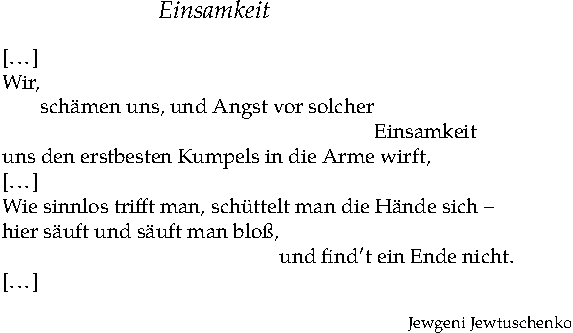
\includegraphics{Roemer-Beispiel3-crop}
\end{center}

Mit der Umgebung \texttt{altverse} können individuell gestaltete Strophen gesetzt werden; sie hat den Effekt, dass z.\,B. bei den paarweise 
strukturierten
Strophen die 2., 4. etc. Zeile um die Länge \verb|\vgap| einrückt.
Als Alternative wird für die \texttt{verse}-Umgebung der Einschluss einzelner
Verse in die \texttt{patverse}-Umgebung angeboten.

\begin{center}
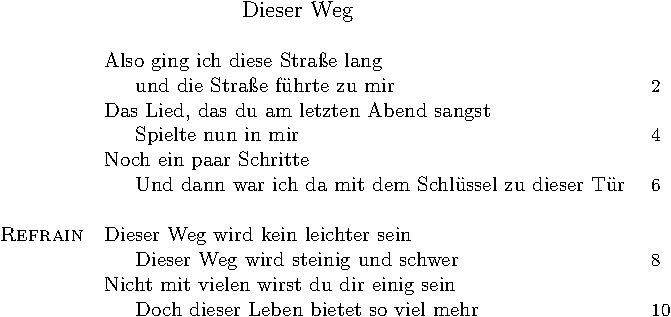
\includegraphics{Roemer-Beispiel-crop}
\end{center}

\begin{lstlisting}
\documentclass[ngerman,a4paper,article]{memoir}
[...]
\settowidth{\versewidth}{Das Lied, das du am letzten Abend sangst}
\PoemTitle*{Dieser Weg}
\begin{verse}[\versewidth]
\linenumberfrequency{2}
\begin{altverse}
  Also ging ich diese Straße lang\\
  und die Straße führte zu mir\\
  Das Lied, das du am letzten Abend sangst\\
  Spielte nun in mir\\
  Noch ein paar Schritte\\
  Und dann war ich da mit dem Schlüssel zu dieser Tür\\!
\end{altverse}

\begin{altverse}
\flagverse{\textsc{Refrain}\quad} Dieser Weg wird kein leichter sein\\
  Dieser Weg wird steinig und schwer\\
  Nicht mit vielen wirst du dir einig sein\\
  Doch dieser Leben bietet so viel mehr\\
\end{altverse}
\linenumberfrequency{0}
\end{verse}
\end{lstlisting}

Das neue poetrytex-Paket von Sam Whited (Juli 2012) ist primär für das Setzen
von poetischen Anthologien geschaffen worden. Die verse-Umgebung wurde darin
etwas modifiziert und in eine \texttt{poem}-Umgebung umgebaut.


\subsection{Darstellen von Reim, Rhythmus und Metrum}

Klassische Gedichte reimen nach bestimmten Schemata. So nennt man beispielsweise
ein Gedicht aus Vierzeilern Quartett. Wenn sich die ersten und die beiden letzten
Zeilen jeweils beim Aussprechen reimen, wird dies als Paarreim bezeichnet. 
Wenn sich das Ende von Verszeilen reimt, ist dies ein Endreim, den es wieder in
verschiedenen Ausprägungen gibt. Veranschaulicht wird dies in der Regel mit
Kleinbuchstaben:

\begin{tabular}{cl}
aabb & Paarreim \\
abab & Kreuzreim \\
abba & umarmender Reim \\
\ldots & \ldots \\
\end{tabular}

Rhythmus und Metrum werden auch Versmaß genannt. Die regelmäßige Abfolge von betonten
und unbetonten Silben ist der Rhythmus, der in der lyrischen Sprache nach einem sich 
wiederholenden Takt (Metrum) aufgebaut sein kann. Eine metrisch gebundene Verszeile 
umfasst mehrere Takte und wird damit als zwei-, drei- oder vierhebig bezeichnet. Man
unterscheidet traditionell nach den Metren verschiedene Rhythmen in den Wortsilben:
den Jambus (unbetont, betont) et cetera. Um mehr Übersichtlichkeit bei der Vermittlung und
Bestimmung des Versmaßes zu bekommen wird die Abfolge von Hebungen und Senkungen auch
graphisch dargestellt. Das übliche Modell nimmt dafür den Backslash (\verb|\|) für eine 
Hebung und "`ein kleines breites U"' ($\cup$) für die Senkung \cite[S.\,17]{Neuhaus}.

Beispielsweise wurde der Daktylus, der schon in der griechischen Ilias Verwendung fand,
während der Klassikepoche in der deutschen Verslehre als Abfolge einer 
betonten und zweier unbetonten Silben definiert.

\begin{tabular}{ll}
betont - unbetont - unbetont: &  \verb|\| $\cup$ $\cup$ \\
\end{tabular}

\begin{lstlisting}
 \verb|\| $\cup$ $\cup$ 
\end{lstlisting}

Um sich die Arbeit etwas zu erleichtern, ist es sinnvoll, Befehle zu definieren.
Es dürfen dafür aber keine Befehle genommen werden, die es schon gibt:
\begin{lstlisting}
\usepackage{xspace}

\newcommand\He{\textbackslash\xspace}%  Hebung
\newcommand\Se{$\cup$\xspace}%  Senkung 
\end{lstlisting}

Der Daktylus tritt in dem folgenden Beispiel auf:

\poemtitle{\textbf{Wür}de der \textbf{Frau}en}
\settowidth{\versewidth}{Ehret die Frauen! sie flechten und weben}
 \poemlines{1} 
\begin{verse}[\versewidth]
\textbf{Eh}ret die \textbf{Frau}en! sie \textbf{flech}ten und \textbf{we}ben\\
\textbf{Himm}lische \textbf{Ro}sen ins \textbf{ir}dische \textbf{Le}ben,\\
\textbf{Flech}ten der \textbf{Lie}be be\textbf{glüc}kendes \textbf{Band},\\
\textbf{Und} in der \textbf{Gra}zie \textbf{züch}tigem \textbf{Schlei}er\\
\textbf{Näh}ren sie \textbf{wach}sam das \textbf{e}wige \textbf{Feu}er\\
\textbf{Schö}ner Ge\textbf{füh}le mit \textbf{hei}liger \textbf{Hand}.\\
\end{verse}
\attrib{Friedrich Schiller}

Das Schema dazu:

\begin{center}

\begin{tabular}{@{}clc@{}}
Vers & Metrum & Reim \\ 
\hline 
  & \He\Se \Se \He\Se \\
1 & \He\Se \Se  \He\Se \Se \He\Se \Se \He\Se  & a\\
2 & \He\Se\Se \He\Se \Se \He\Se\Se \He\Se  & a\\
3 & \He\Se \Se \He\Se \Se\He\Se\Se \He & b\\
4 & \He \Se \Se \He\Se \He\Se\Se \He\Se & c\\
5 & \He\Se \Se \He\Se \Se \He\Se\Se \He\Se & c\\
6 & \He\Se \Se\He\Se \Se \He\Se\Se \He & b\\
\end{tabular}

\end{center}

\begin{lstlisting}
\begin{tabular}{@{}clc@{}}
Vers & Metrum & Reim \\ 
\hline 
 & \He\Se \Se \He\Se \\
1 & \He\Se \Se  \He\Se \Se \He\Se \Se \He\Se  & a\\
2 & \He\Se\Se \He\Se \Se \He\Se\Se \He\Se  & a\\
3 & \He\Se \Se \He\Se \Se\He\Se\Se \He & b\\
4 & \He \Se \Se \He\Se \He\Se\Se \He\Se & c\\
5 & \He\Se \Se \He\Se \Se \He\Se\Se \He\Se & d\\
6 & \He\Se \Se\He\Se \Se \He\Se\Se \He & d\\
\end{tabular}
\end{lstlisting}


Wie zu sehen ist, unterscheiden sich die Verse bei der Betonung der letzten 
Silbe; ist die letzte Silbe im Vers betont, liegt eine männliche, ist sie unbetont
eine weibliche Kadenz
vor. Der Titel, Vers 1, 2, 4, 5 haben weibliche und Vers 3 und 6 haben 
männliche Kadenz.

Wenn man sehen will, wie sich die Hebungen und Senkungen auf die
einzelnen Wörter verteilen, kann der Wortzwischenraum beispielsweise
durch einen Unterstrich markiert werden. Damit keine uneinheitlichen Abstände 
um den Unterstrich entstehen, kann man ein Makro für
den Wortzwischenraum (\verb|Zr|) verwenden:

\verb|\newcommand*{\Zr}{\unskip\textunderscore}|

Würde der Frauen: \He\Se\Zr\Se\Zr\He\Se =\verb|\He\Se\Zr\Se\Zr\He\Se|

%\He\Se\_\Se\_\He\Se \quad = \verb|\He\Se\_\Se\_\He\Se| 


Es ist auch möglich komplexe "`Bausteine"' zu definieren. Beispielsweise
\verb|\daktylus|: \daktylus{} (Daktylus) oder \verb|\anapaest| (Anapäst) 
\anapaest.

\begin{lstlisting}
\newcommand\daktylus{$\textbackslash\cup\cup$\xspace} 
\newcommand\anapaest{$\cup\cup\textbackslash$\xspace} 
\end{lstlisting}

\small
\begin{thebibliography}{1000}
\bibitem
{Neuhaus} Stefan Neuhaus:
\textsl{Grundriss der Literaturwissenschaft}. 
A. Francke Verlag: Tübingen und Basel, 3. überarbeitete und erweiterte Auf\/lage, 
2009.

\bibitem
{Svoboda} Atze Svoboda:
\textsl{Was gesagt werden muss}.
In: Eulenspiegel, Heft 5/2012, S.\,14.

\bibitem
{Willberg} Hans Peter Willberg /Friedrich Forsman:
\textsl{Lesetypografie.}
Verlag Hermann Schmidt: Mainz 2010.

\bibitem
{wilson} Peter R. Wilson/Lars Madsen:
\textsl{The Memoir Class for Configurable Typesetting. User Guide.}
The Herries Press, Normandy Park, WA 2011.
\url{macros/latex/contrib/memoir/memman.pdf}.

\bibitem
{Wilson} Peter R. Wilson:
\textsl{Typesetting simple verse with \LaTeX }. 2004.
\url{macros/latex/contrib/verse/verse.pdf}
\end{thebibliography}

%\end{document}



%\end{document}
